%%%%%%%%%%%%%%%%%%%%%%%%%%%%%%%%%%%%%%%%%
% Friedrich M. Grabner - 01220997
% HPC Coursework
%%%%%%%%%%%%%%%%%%%%%%%%%%%%%%%%%%%%%%%%%

%----------------------------------------------------------------------------------------
%	PACKAGES AND DOCUMENT CONFIGURATIONS
%----------------------------------------------------------------------------------------
\documentclass[10pt, a4paper]{article}
\usepackage{amsmath, amsthm, amssymb}
\usepackage{graphicx} % Required for the inclusion of images
\usepackage{natbib} % Required to change bibliography style to APA
\usepackage{nomencl}
\usepackage{setspace}
\usepackage{geometry} 
\usepackage{hyperref}
\usepackage{subcaption}
\usepackage{xcolor}
\usepackage{lmodern}
\usepackage{listings}
\lstset{language=[90]Fortran,
  basicstyle=\ttfamily,
  keywordstyle=\color{red},
  commentstyle=\color{green},
  morecomment=[l]{!\ }% Comment only with space after !
}

\geometry{a4paper,total={170mm,257mm},left=20mm,top=20mm}



\setlength\parindent{5pt} % Removes all indentation from paragraphs
\graphicspath{{./images/}}
\DeclareGraphicsExtensions{.pdf,.PDF,.jpg,.JPG,.bmp,.png,.eps,.EPS}

%\usepackage{times} % Uncomment to use the Times New Roman font

\input{/home/fmg215/Documents/latex/symbols.tex}
%----------------------------------------------------------------------------------------
%	DOCUMENT INFORMATION
%----------------------------------------------------------------------------------------
\newcommand*{\plogo}{\fbox{$\mathcal{PL}$}}

\newcommand*{\titleGM}{\begingroup % Create the command for including the title page in the document
\hbox{ % Horizontal box
\hspace*{0.2\textwidth} % Whitespace to the left of the title page
\rule{1pt}{\textheight} % Vertical line
\hspace*{0.05\textwidth} % Whitespace between the vertical line and title page text
\parbox[b]{0.75\textwidth}{ % Paragraph box which restricts text to less than the width of the page

{\noindent\huge\bfseries High Performance Computing \\[0.5\baselineskip] AE3-422}\\[2\baselineskip] % Title
{\Large \textsc{F. M. Grabner - 01220997}}\\[4\baselineskip] % Tagline or further description
{\large } % Author name

\vspace{0.5\textheight} % Whitespace between the title block and the publisher
{\noindent Imperial College London - Department of Aeronautics}\\[\baselineskip] % Publisher and logo
}}
\endgroup}
%----------------------------------------------------------------------------------------
%	TITLE PAGE
%----------------------------------------------------------------------------------------
\begin{document}
\titleGM
%----------------------------------------------------------------------------------------
%	QUESTION 1
%----------------------------------------------------------------------------------------
\section*{Question 1}
Figure \ref{fig:task1} shows the analytical solution against computed solution using the static equations. The computed solution shows strong correlation to that of the analytical.

\begin{figure}[!htb]
  \centering
	  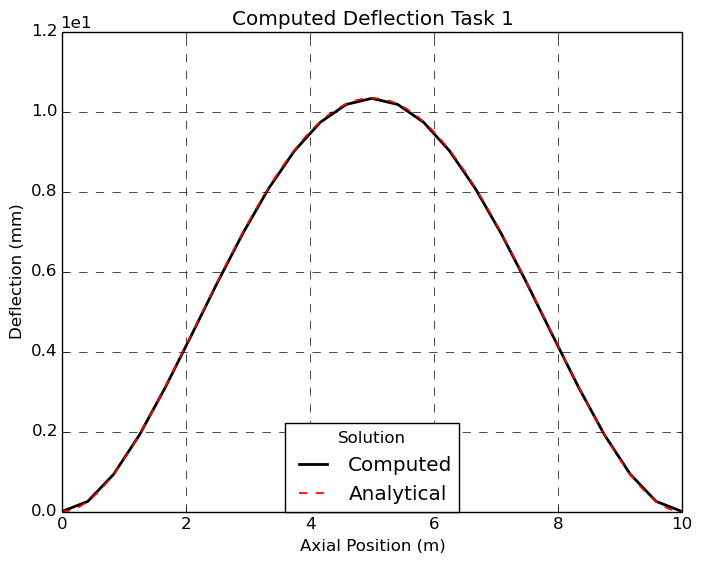
\includegraphics[width=.75\linewidth, clip=true, trim=0cm 0cm 0cm 0cm]{task1}
  \caption{Static against analytical solutions.}
  \label{fig:task1}
\end{figure}%

Matrices have been set up in banded format to minimise the memory footprint. Then the system is solved utilising Lapack\cite{Lapack1999} function DGBSV. However to utilise the Fortran routines in BLAS\cite{Blas1979}, column-major storage format has been utilised which goes against natural C++ format.

%----------------------------------------------------------------------------------------
%	QUESTION 2
%----------------------------------------------------------------------------------------
\section*{Question 2}

%---------------------------------------------------------------------------------------
%	BIBLIOGRAPHY
% ---------------------------------------------------------------------------------------
\bibliographystyle{unsrt}	% in order of appearance
%\bibliographystyle{acm}	% (uses file "plain.bst")
%\bibliographystyle{abbrv}	% (uses file "plain.bst")
%\bibliographystyle{siam}	% (uses file "plain.bst")
%\bibliographystyle{apalike}
\bibliography{/home/fmg215/Documents/latex/myrefs}		% expects file "myrefs.bib"}
%----------------------------------------------------------------------------------------
% END DOCUMENT
%----------------------------------------------------------------------------------------
\end{document}